Die Grenzfrequenz $f_{gr}$ ist die Frequenz, bei der die Übertragungsfunktion
(Verstärkung) den Wert $\frac{1}{\sqrt{2}}$ annimmt (Abfall von
$-3\,\si{\deci\bel}$).

Die Bandbreite $B$ ist die Differenz zwischen niedrigster und
höchster Frequenz, welche eine Dämpfung von $\frac{1}{\sqrt{2}}$ aufweisen.

Die Güte ist der Quotient aus Mittenfrequenz $f_0$ und Bandbreite $B$ eines
Bandpasses. Sie ist ein Maß für dessen Steilheit.

\subsubsection{Tiefpass 1. Ordnung}

\begin{figure}[H]
  \begin{center}
    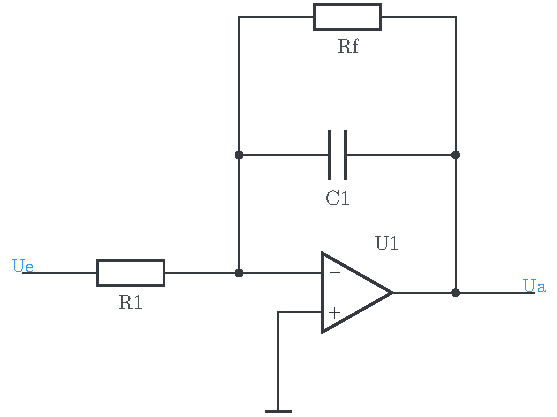
\includegraphics[width=0.618\textwidth]{circuits/tp.pdf}
  \end{center}
  \caption{Tiefpass 1. Ordnung}
\end{figure}

\begin{gather*}
  \frac{u_a}{u_e} = V(\omega) = -\frac{Z_2}{Z_1} = -\frac{R_f // \frac{1}{j \omega
    C_1}}{R_1}\\
= -\dfrac{ \dfrac{R_f \cdot \frac{1}{j\omega C_1}}{R_f + \frac{1}{j \omega C_1}}}{R_1}
\end{gather*}
\eqbox{
  V(\omega) = -\frac{R_f}{R_1} \cdot \frac{1}{1 + j \omega R_f C_1}
}{0.618\textwidth}

\eqbox{
  |V(\omega)| = \frac{R_f}{R_1} \cdot \frac{1}{\sqrt{1 + \omega^2 R_f^2 C_1^2}}
}{0.618\textwidth}

\eqbox{
  \phi(\omega) = -\arctan{\omega R_f C_1}
}{0.618\textwidth}

\begin{figure}[H]
  \begin{center}
    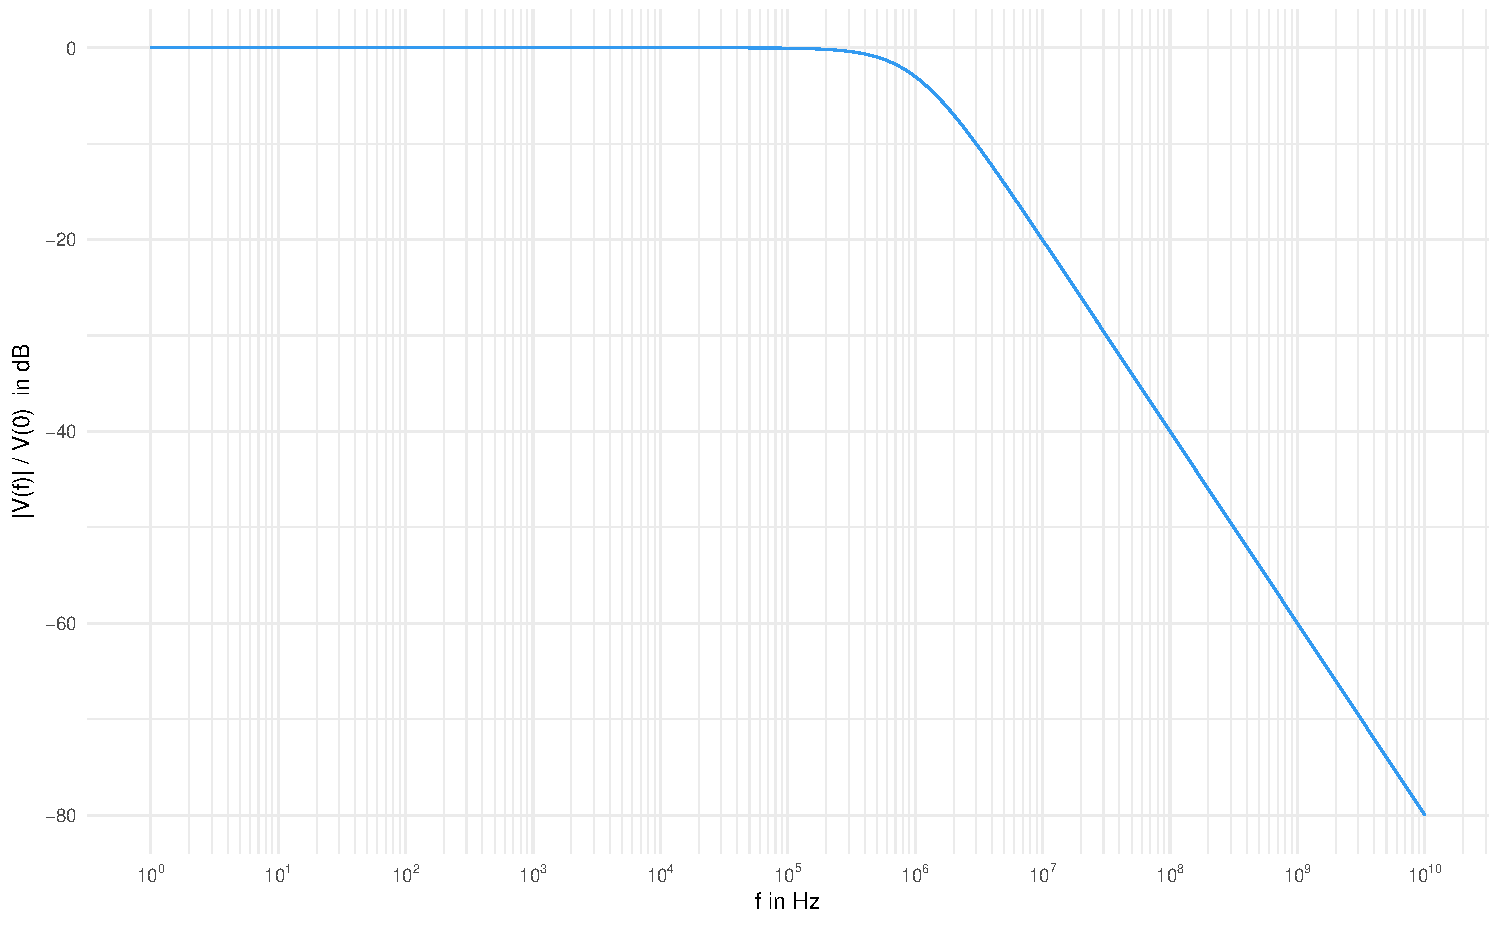
\includegraphics[width=\textwidth]{1_10/TP/TP.pdf}
  \end{center}
  \caption{Beispielhafter (normierter) Betragsfrequenzgang des Tiefpasses}
\end{figure}

\begin{figure}[H]
  \begin{center}
    \includegraphics[width=\textwidth]{1_10/TP/PH.pdf}
  \end{center}
  \caption{Beispielhafter Phasengang des Tiefpasses}
\end{figure}

\subsubsection{Hochpass 1. Ordnung}

\begin{figure}[H]
  \begin{center}
    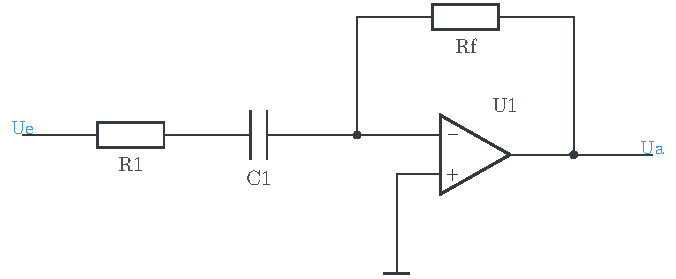
\includegraphics[width=0.618\textwidth]{circuits/hp.pdf}
  \end{center}
  \caption{Hochpass 1. Ordnung}
\end{figure}

\begin{gather*}
  \frac{u_a}{u_e} = V(\omega) = -\frac{Z_2}{Z_1} = -\frac{R_f}{R_1 +
    \frac{1}{j\omega C_1}}\\
\end{gather*}
\eqbox{
  V(\omega)=\frac{R_f}{R_1} \cdot \dfrac{1}{1+\dfrac{1}{j\omega R_1 C_1}}
}{0.618\textwidth}

\eqbox{
  |V(\omega)|=\frac{R_f}{R_1} \cdot \dfrac{1}{\sqrt{1+\dfrac{1}{\omega^2 R_1^2 C_1^2}}}
}{0.618\textwidth}

\eqbox{
  \phi(\omega) = \arctan{\frac{1}{\omega R_1 C_1}}
  }{0.618\textwidth}

\begin{figure}[H]
  \begin{center}
    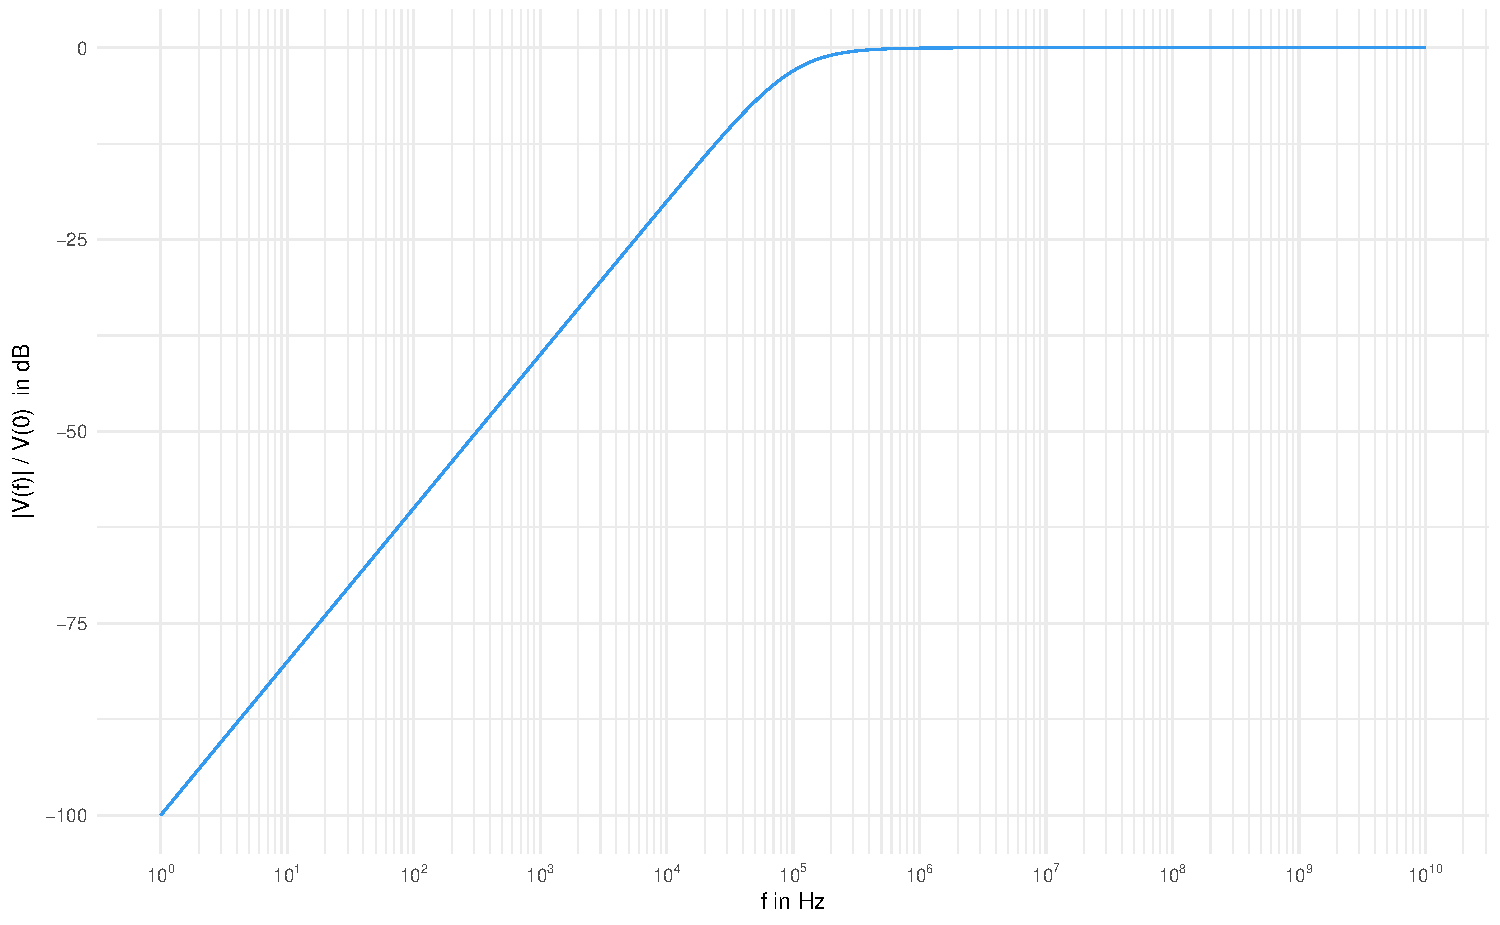
\includegraphics[width=\textwidth]{1_10/HP/HP.pdf}
  \end{center}
  \caption{Beispielhafter (normierter) Betragsfrequenzgang des Hochpasses}
\end{figure}

\begin{figure}[H]
  \begin{center}
    \includegraphics[width=\textwidth]{1_10/HP/PH.pdf}
  \end{center}
  \caption{Beispielhafter Phasengang des Hochpasses}
\end{figure}

\subsubsection{Bandpass 1. Ordnung}
\begin{figure}[H]
  \begin{center}
    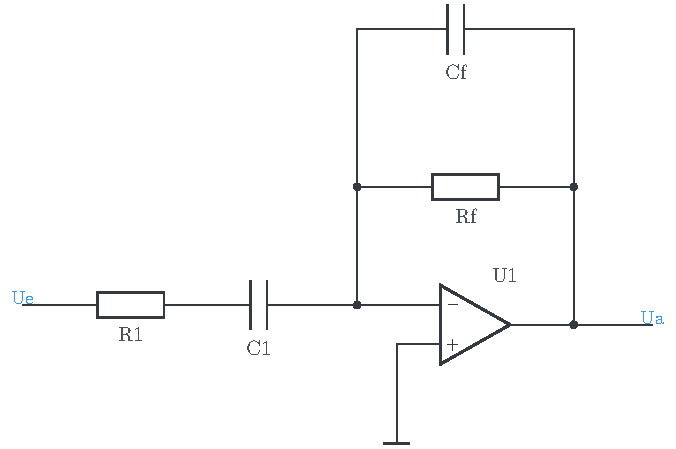
\includegraphics[width=0.618\textwidth]{circuits/bp1.pdf}
  \end{center}
  \caption{Bandpass 1. Ordnung}
\end{figure}

\begin{gather*}
  \frac{u_a}{u_e} = V(\omega) = -\frac{Z_2}{Z_1} = -\frac{R_f // \frac{1}{j \omega
    C_f}}{R_1 // \frac{1}{j \omega C_1}}\\
= - \dfrac{ \dfrac{R_f \cdot \frac{1}{j \omega C_f}}{R_f + \frac{1}{j \omega
      C_f}} }{ R_1 + \frac{1}{j \omega C_1} }
= - \dfrac{ \dfrac{R_f}{1 + j \omega R_f C_f} }{ R_1 + \frac{1}{j \omega C_1}
}\\
\end{gather*}
\eqbox{
V(\omega) = - \frac{R_f}{R_1} \cdot \frac{1}{\left( 1 + j \omega R_f C_f \right) \cdot
  \left( 1 + \dfrac{1}{j \omega R_1 C_1}\right) }
}{0.618\textwidth+1.6cm}

\eqbox{
|V(\omega)| = \frac{R_f}{R_1} \cdot \frac{1}{\sqrt{\left( 1 + \frac{R_f
        C_f}{R_1 C_1}\right)^2 \cdot
  \left( \omega R_f C_f - \frac{1}{\omega R_1 C_1}\right)^2 }}
}{0.618\textwidth+1.6cm}

\eqbox{
\phi(\omega) = \arctan{ \frac{\omega R_f C_f - \dfrac{1}{\omega R_1 C_1}}{1 +
    \dfrac{R_f C_f}{R_1 C_1}} }
}{0.618\textwidth+1.6cm}

\begin{figure}[H]
  \begin{center}
    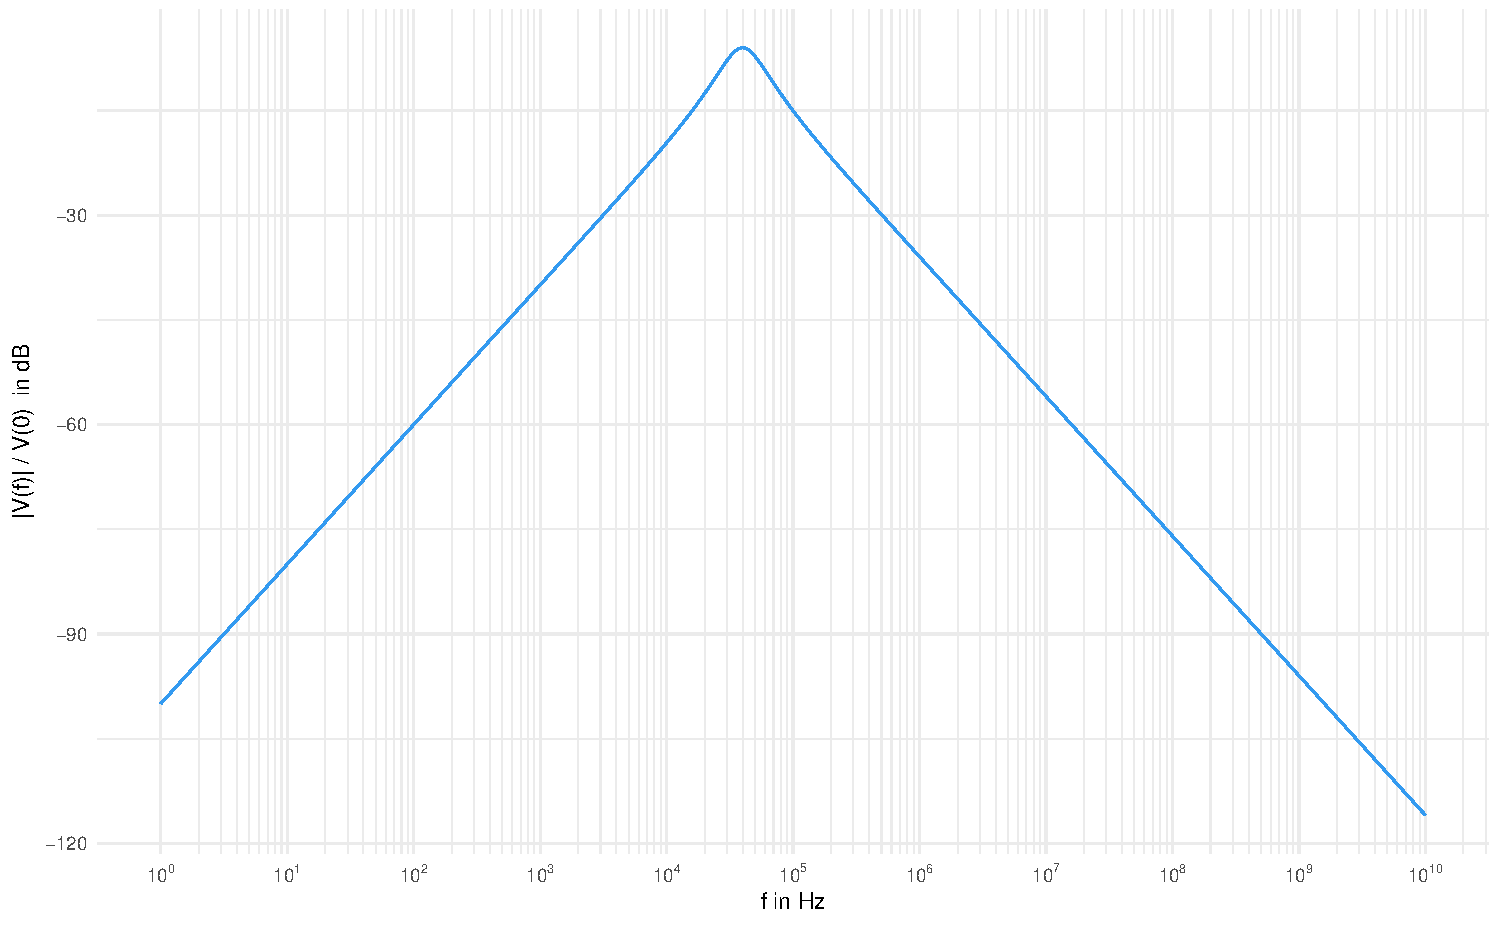
\includegraphics[width=\textwidth]{1_10/BP1/BP.pdf}
  \end{center}
  \caption{Beispielhafter (normierter) Betragsfrequenzgang des Bandpasses 1. Ordnung}
\end{figure}

\begin{figure}[H]
  \begin{center}
    \includegraphics[width=\textwidth]{1_10/BP1/PH.pdf}
  \end{center}
  \caption{Beispielhafter Phasengang des Bandpasses 1. Ordnung}
\end{figure}


\subsubsection{Bandpass 2. Ordnung}

\begin{figure}[H]
  \begin{center}
    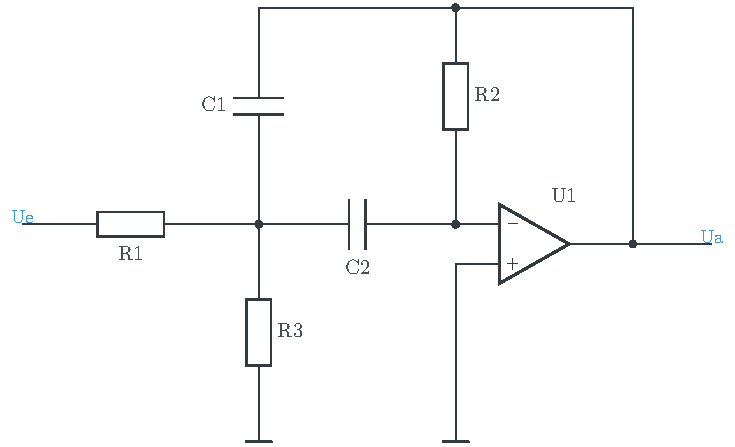
\includegraphics[width=0.618\textwidth]{circuits/bp2.pdf}
  \end{center}
  \caption{Bandpass 2. Ordnung}
\end{figure}

\begin{center}
\eqbox{
  |V(\omega)| = \dfrac{R_2 C_2}{\sqrt{ (R_1(C_1+C_2))^2 + \left(
        \dfrac{1}{\omega} \left(1 + \dfrac{R_1}{R_3} \right) - \omega
        R_1 C_1 R_2 C_2 \right)^2} } 
}{\textwidth}
\end{center}